\chapter{Proof of concept}
\label{ch:proofofconcept}

\section{Inleiding}

Nu we een duidelijker beeld hebben van de hard- en software die op dit moment op de markt beschikbaar is alsook hoe we dit concept zouden kunnen implementeren, kunnen we dit deels uitwerken in de vorm van een scenario.
Het scenario begint op het moment waar een bemanningslid (of klant in het geval van cruiseschepen) overboord gevallen is. De eerste reactie van het bevoegd personeel is om de drone uit te halen en volledig voor te bereiden voor vertrek alsook de reddingsdiensten te contacteren en over het incident in te lichten. Op die manier kunnen de reddingsdiensten zo snel mogelijk vertrekken.
Na het inlichten van de reddingsdiensten begint onze test. 

Beeldmateriaal van het experiment kan bekeken worden via volgende link:\newline
https://youtu.be/jnHxVoWearw

\section{Situering van de test}

Zoals hierboven vermeld werd, zitten we dus volgens ons scenario op een groot schip zoals bijvoorbeeld een vracht- of cruiseschip. Door één of ander ongelukkig ongeval is er een werknemer of klant van het dek afgevallen en ligt nu in het water. De werknemers of passagiers hebben dit doorgegeven aan de kapitein en deze is nu bezig met het stil leggen van het schip. Ondertussen is een werknemer die hiervoor getraind werd en dus de nodige kennis heeft, de drone aan het voorbereiden voor vertrek. In onze test maken we gebruik van de DJI Mavic Pro (figuur \ref{drone}. Deze drone kan bestuurd worden aan de hand van zowel iOS als android apps. Voor onze test gebruiken we de DJI GO 4 app en de Litchi app die beide over een aantal handige functionaliteiten beschikken.

\begin{figure}[h]
	\centering
	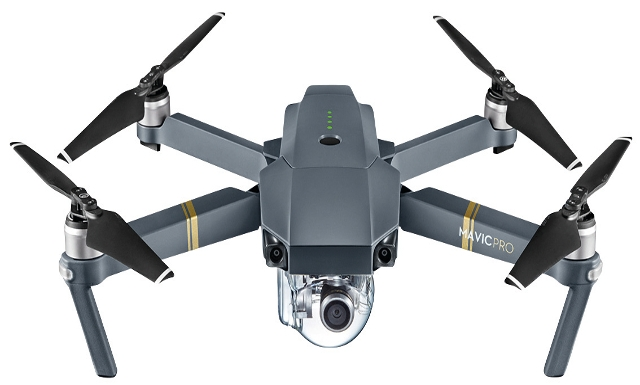
\includegraphics[width=.8\textwidth]{drone}
	\caption{DJI Mavic Pro \autocite{MavicProImage}}
	\label{drone}
\end{figure}

\newpage
\section{Voorbereiding van de software}

Na het klaar zetten van de drone, neemt de piloot de afstandsbediening en tablet bij zich en opent hij de reeds geïnstalleerde app Litchi. Nadat de app geopend is, navigeert hij naar de "Waypoint" modus waarin hij, manueel of bij voorkeur aan de hand van een template omdat dat sneller is, de verschillende navigatiepunten instelt (figuur \ref{waypoint}). Indien men een goed idee heeft van waar de drenkeling zich bevindt, kan men deze waypoints aanpassen zodat de drone meteen in de juiste richting vliegt. Een alternatief zou kunnen zijn om in alsmaar verder uitdeinende concentrische cirkels rond het schip te circuleren met de drone. Wanneer het pad ingesteld is, drukt men op de "play" toets waarna de drone automatisch dit pad zal volgen. In onze test wordt geopteerd voor een eenvoudige lus vanwege plaatsgebrek maar dit zal in het midden van de oceaan uiteraard niet het geval zijn. 

\begin{figure}[h]
	\centering
	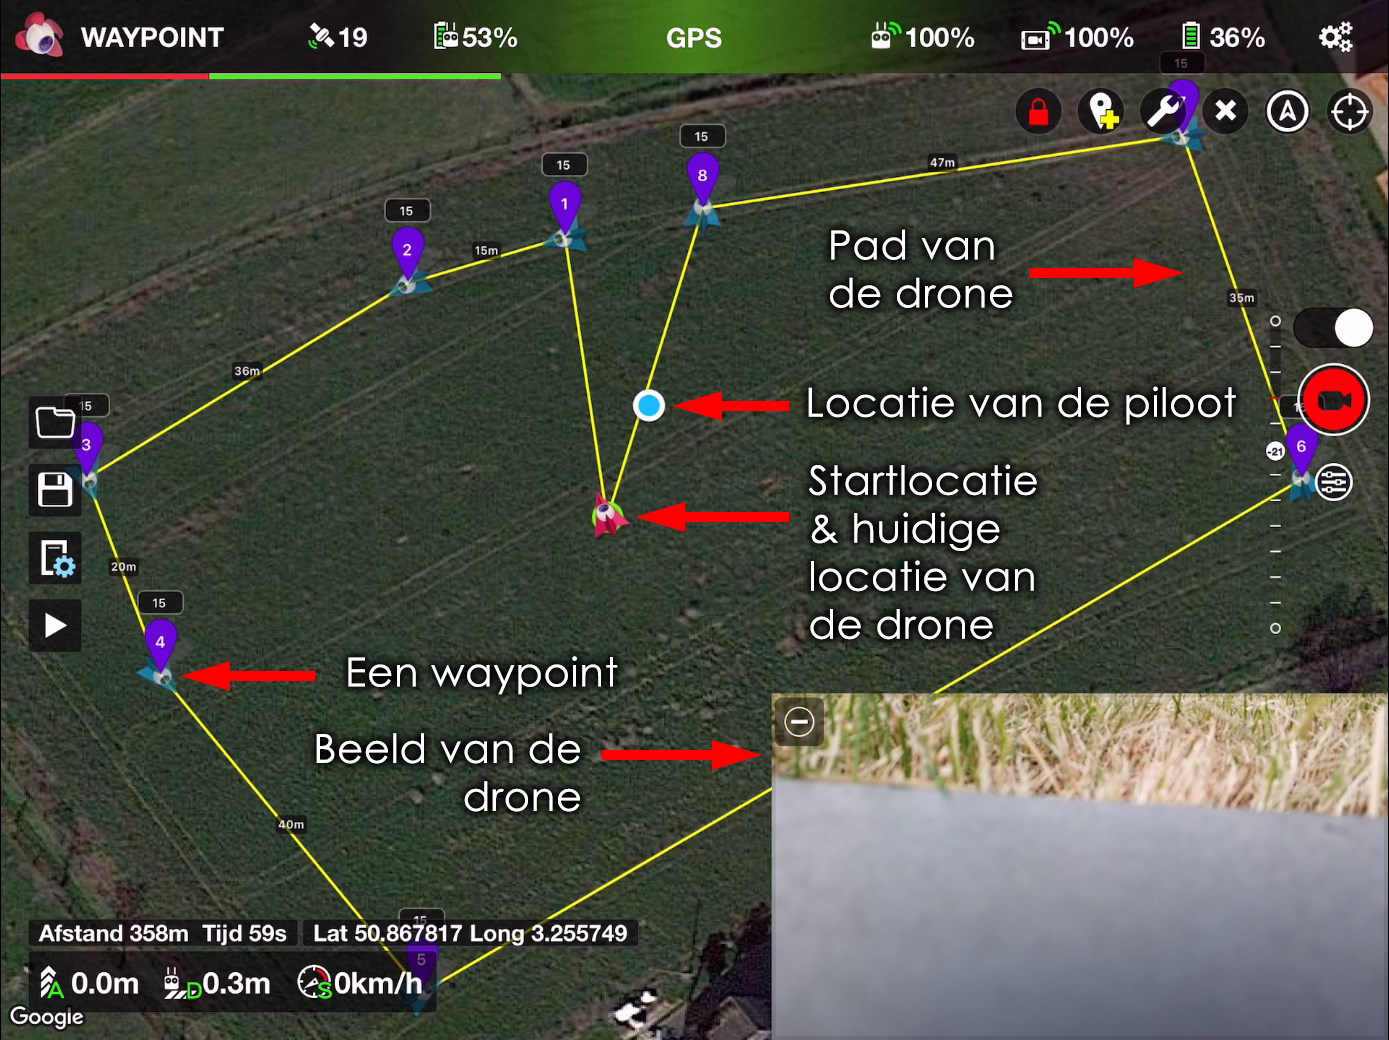
\includegraphics[width=.8\textwidth]{WAYPOINT}
	\caption{Een kaart van de locatie met de waypoints erop aangeduid}
	\label{waypoint}
\end{figure}


\section{Tijdens de vlucht}

De drone is nu vertrokken en volgt autonoom het ingestelde pad dankzij de Litchi app. Hoewel het detecteren van een drenkeling via de SDK (gemaakt en ter beschikking gesteld door DJI) wel geautomatiseerd zou kunnen worden, gaan wij gedurende de test op het zicht kijken wanneer de drenkeling op het scherm in beeld komt. In onze test is dit met een gewone camera wat op zich niet altijd de optimale oplossing is in donkere omstandigheden of in klaarlichte dag maar als we gebruik zouden maken van infra-rood en/of warmte camera's, zoals eerder besproken werd in hoofdstuk 2 en 3, dan zou het verschil tussen de drenkeling en de omgeving (oceaan) duidelijk genoeg zijn zodat dit geen probleem meer vormt.

\section{Gevonden!}

We hebben de drenkeling gevonden zoals je kan zien op figuur \ref{far}! Op dit moment moet de verantwoordelijke, de besturing van de drone even overnemen om hem correct te positioneren (figuur \ref{close}) waarna hij de "Active Tracking" functie kan activeren (figuur \ref{funcswitch}). Het exact positioneren van de drone zou opnieuw geautomatiseerd kunnen worden maar dit doen we in onze test niet. De "Active Tracking" functie is in staat om een object, dat aangeduid werd door de gebruiker, te volgen en in het midden van het beeld te houden (figuur \ref{activetrack}). Dan moet de crew van het schip slechts de coördinaten, die ze op het scherm waarop de app draait kunnen aflezen, door te geven aan de reddingsdiensten zodat zij een exacte locatie hebben om naartoe te navigeren. Van zodra de reddingsdiensten ter plaatse zijn, is het de taak van de bestuurder van de drone om deze op tijd weg te navigeren van de drenkeling zodat de reddingsoperatie niet bemoeilijkt wordt.

\newpage

\begin{figure}[h]
	\centering
	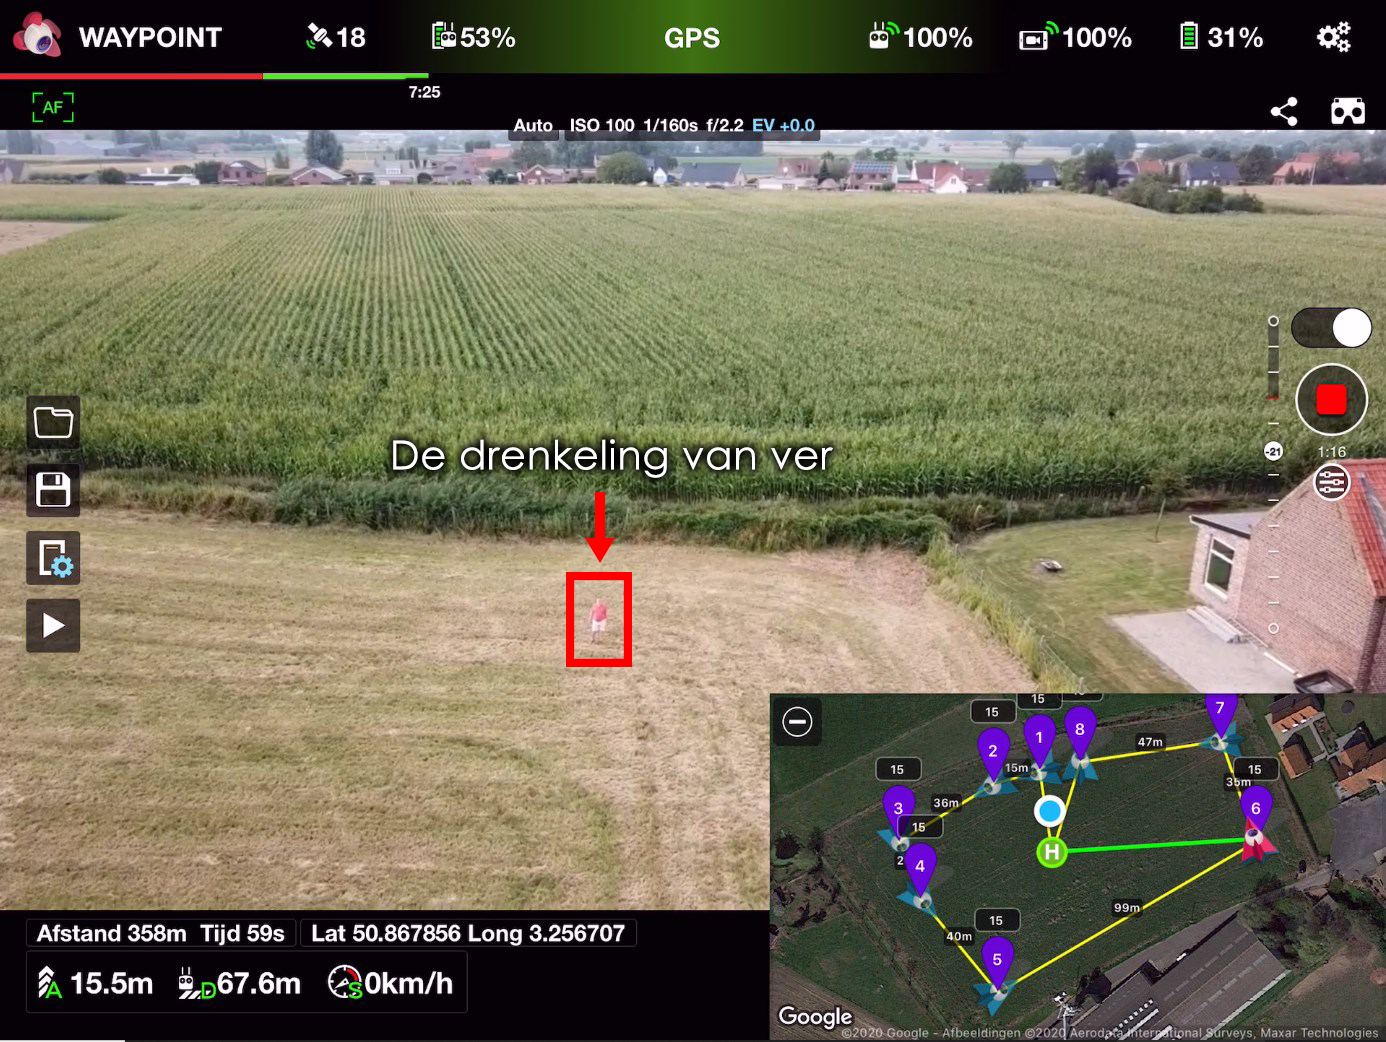
\includegraphics[width=.7\textwidth]{DRENKELING_VER}
	\caption{De drenkeling wanneer hij van ver gezien wordt.}
	\label{far}
\end{figure}
\begin{figure}[h]
	\centering
	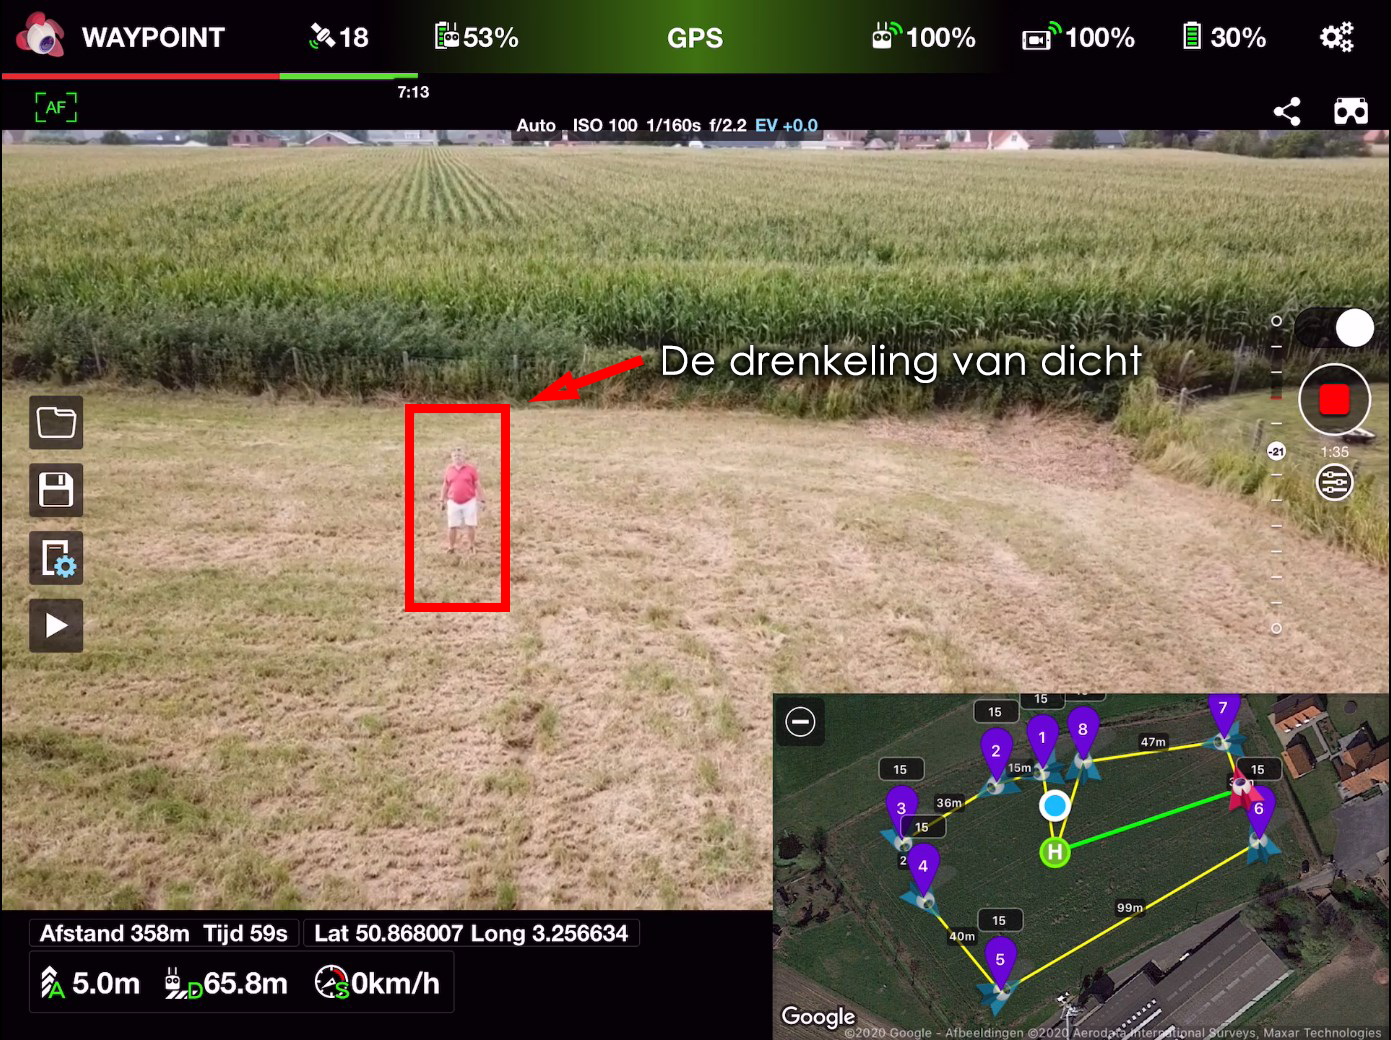
\includegraphics[width=.7\textwidth]{DRENKELING_DICHT}
	\caption{De drenkeling nadat de drone correct gepositioneerd is.}
	\label{close}
\end{figure}

\newpage

\begin{figure}[h]
	\centering
	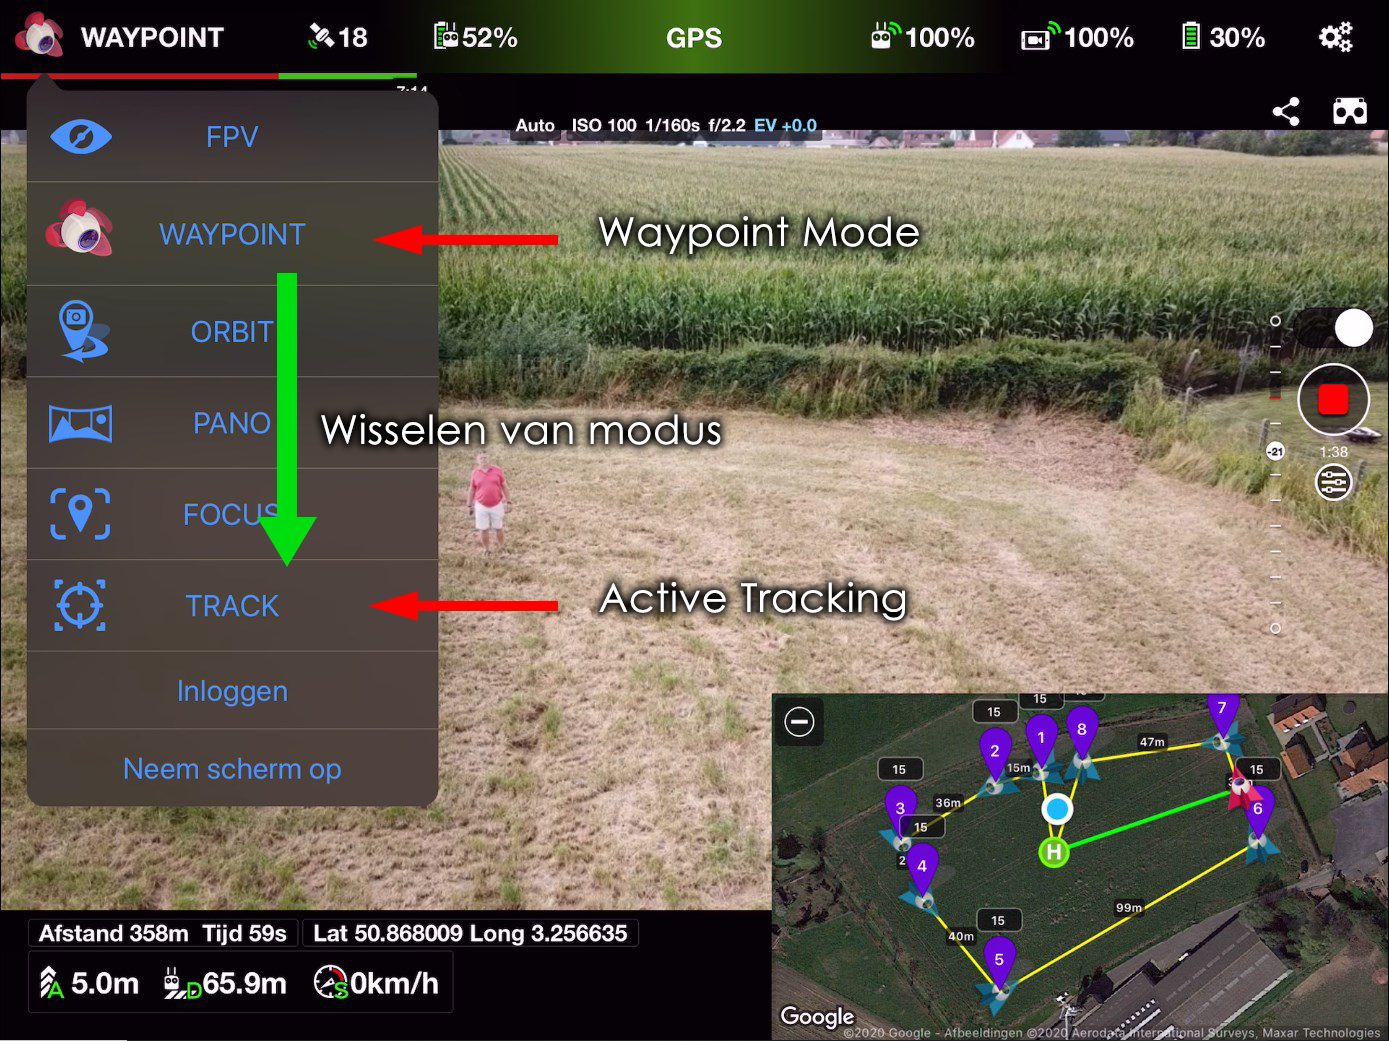
\includegraphics[width=.7\textwidth]{FUNCTIONALITEITEN}
	\caption{Het functionaliteitenmenu van de Litchi app. Bevat o.a. waypoint en tracking}
	\label{funcswitch}
\end{figure}
\begin{figure}[h]
	\centering
	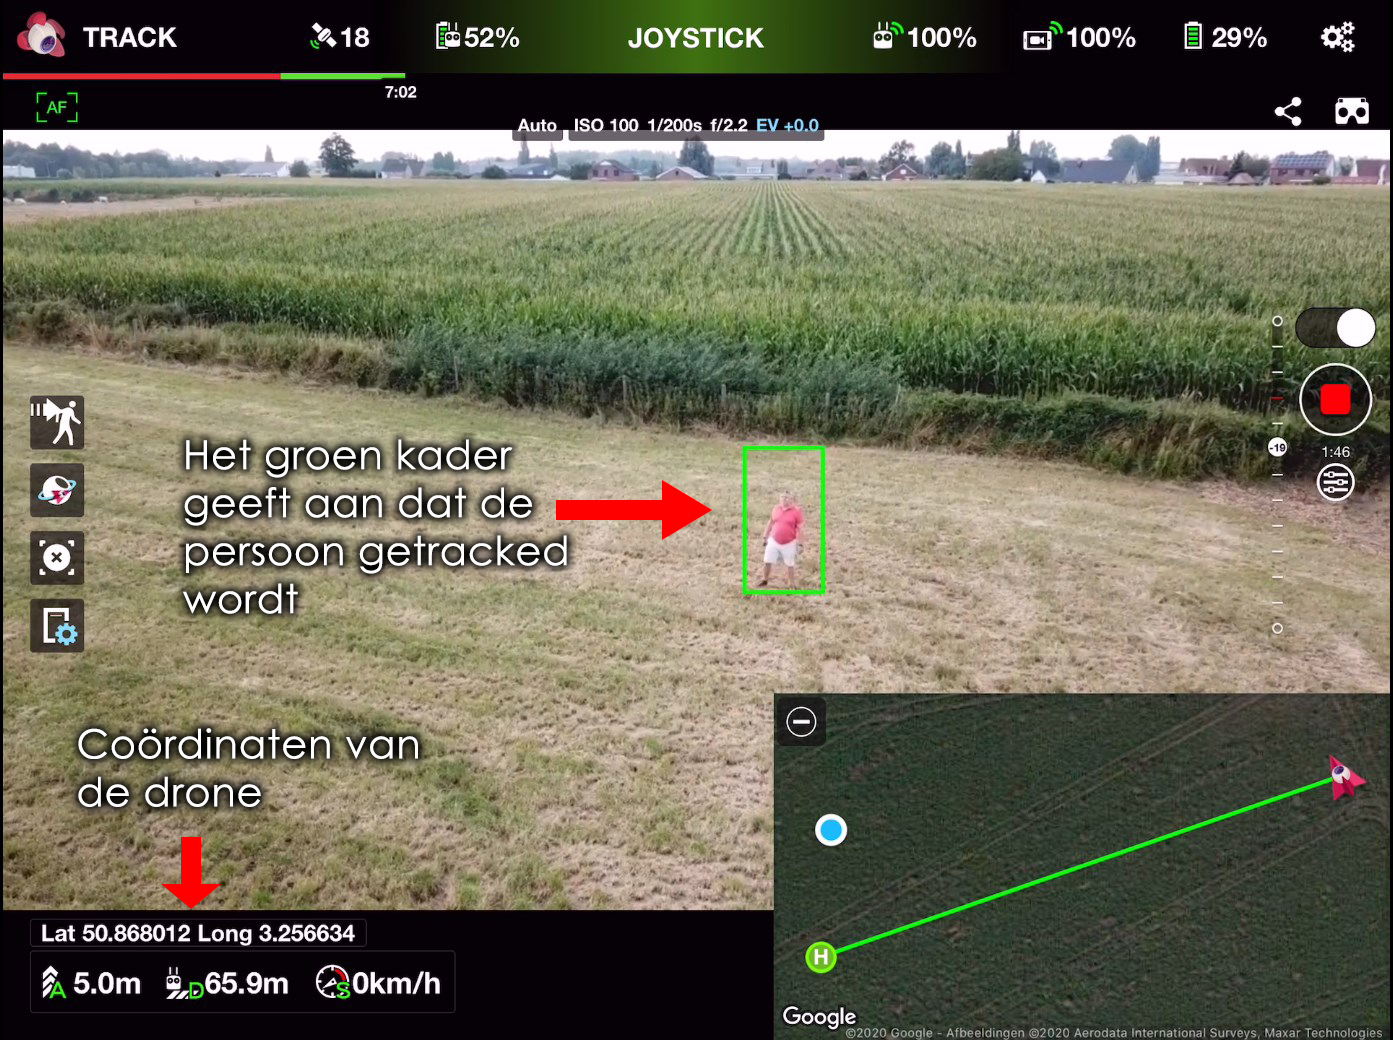
\includegraphics[width=.7\textwidth]{ACTIVE_TRACKING}
	\caption{De app tijdens active tracking}
	\label{activetrack}
\end{figure}

\newpage

\section{Bevindingen}

Tijdens het uitvoeren van ons scenario hebben we het volgende vastgesteld:

\begin{itemize}
	\item De ''Waypoint'' functionaliteit van de Litchi app werkte heel erg goed. De drone was in staat om het vooraf ingestelde pad zonder problemen te volgen.
	\item De ''Active Tracking'' functionaliteit van de Litchi app werkte niet zo goed. Het verloor zijn ''zicht'' op de drenkeling na enkele seconden waardoor we het kader rond de ''drenkeling'' ook dikwijls moesten hertekenen.
\end{itemize}

Wil dit dan zeggen dat ''Active Tracking'' een technologie is die nog niet op punt staat? Nee, het werkt namelijk perfect op de app die door DJI zelf ontwikkeld is. Zelfs op een hoogte van 10-15 meter, wanneer het lichaam van een persoon veel kleiner is, kon de drone onze drenkeling nog steeds volgen en in beeld houden. Het is dus vooral de Litchi Active Tracking die nog geoptimaliseerd moet worden. Ondanks het feit dat de technologie nog niet helemaal op punt staat, zijn er duidelijk mogelijkheden genoeg die voldoen aan de vereisten van onze toepassing.